\chapter{Implementation}\label{chapter:implementation}
This chapter covers the details of implementing our prototype regular expressions engine. The engine takes an input file and a regular expression pattern that is transformed into efficient machine code and dynamically executed on each line of the input file using LLVM JIT Compiler. The prototype is developed using C++ and can be found on Github \footnote{\url{https://github.com/melzareix/jit-regex}}.

\section{System Architecture}
The prototype includes a regular expressions engine, A Command Line Interface (CLI) application to interact with the engine, a benchmark suite, and scripts to generate the data and cases for the benchmarks. We discuss the benchmarks in detail in Chapter \ref{chapter:evaluation}.  The engine is meant to be used as a sub-engine inside an RDBMS (Relational Database Management System) to provide the functionality of regular expressions matching quickly and efficiently. The high-level system architecture of the engine is shown in Figure \ref{fig:sa}.

The inputs to the engine illustrated as yellow boxes in Figure \ref{fig:sa} are (1) a regular expression pattern to compile and (2) an input file or string to search for the pattern inside (3) Optionally several configuration arguments to control the behavior of the engine that are summarized in Table \ref{tab:cliconf}. 

{\renewcommand{\arraystretch}{1.5}% for the vertical padding
\begin{table}[htpb]
\centering
\begin{adjustbox}{width=\textwidth,center=\textwidth}
\small
\begin{tabularx}{\textwidth}{|l|X|l|}
\hline
Option        & Description & Default  \\
\hline
Codegen backend & The Codegen backend to use. Possible values: \texttt{\textbf{LLVM}} or \texttt{\textbf{CPP}}. & \texttt{\textbf{LLVM}}\\
\hline
Bytedfa & If true the DFA is UTF-8 encoded otherwise it uses UTF-32. & \texttt{\textbf{false}} \\
\hline
AsciiEncoding & If true disables Unicode handling in the generated code. & \texttt{\textbf{false}} \\
\hline
OptimizationLevel & Optimization Level for LLVM optimizer (or clang for C++). Possible values: \{\texttt{\textbf{O0,O1,O2,O3,Os,Oz}}\}. & \texttt{\textbf{O2}}\\
\hline
\end{tabularx}
\end{adjustbox}
\caption[CLI Configuration Options]{CLI Configuration Options.}\label{tab:cliconf}
\end{table}}

The engine validates the pattern, parses it, and generates a parse tree. We discuss the implementation of the parser in detail in Section \ref{section:parser}. The DFA Generator checks the pattern if it is simple enough to delegate it to a more efficient matcher. The matcher uses the SIMD instruction set to provide a faster way to match simple literals. We describe the SIMD matcher in detail in Section \ref{section:simdopt}.

If the pattern simplicity check fails, the DFA generator traverses the parse tree and produces a minimal DFA that can recognize the regular expression. The \texttt{\textbf{CodeGen}} module converts the DFA to efficient LLVM IR after that. The LLVM JIT Compiler compiles the IR and returns a function pointer for matching the compiled pattern against the input file.

\begin{figure}[htbp]
    \centering
    \begin{tikzpicture}[->,>=stealth',shorten >=1pt,auto,node distance=1.1cm, scale = 1,transform shape]
        \node (start) [io] {Regular Expression};
        \node (parser) [process, below=of start] {Parser};
        \node (dfa) [process, below=of parser] {DFA Generator};
        \node (dec1) [decision, below=of dfa, align=left] {Simple\\pattern?};
        \node (simd) [process, right=of dec1] {SIMD Matcher};
        \node (codegen) [process, below=of dec1] {CPP\textbackslash LLVM Codegen};
        \node (jit) [process, below=of codegen] {LLVM JIT Compiler};
        \node (cmp) [process2, below=of jit, align=left] {Compiled Regex\\Matcher Function};
        \node (res) [startstop, below=of cmp] {Matching Results};
        
        \node (inpf) [io, right=of cmp] {Input File};
        \node (config) [io, left=of dec1] {Engine Config};
        
    \draw [arrow] (start) -- node[anchor=east] {} (parser);
    \draw [arrow] (parser) -- node[anchor=center,fill=white] {Parse tree} (dfa);
    \draw [arrow] (dfa) -- node[] {} (dec1);
    \draw [arrow] (dec1) -- node[anchor=center,fill=white] {yes} (simd);
    \draw [arrow] (dec1) -- node[anchor=center,fill=white] {no} (codegen);
    \draw [arrow] (codegen) -- node[anchor=center,fill=white] {LLVM IR} (jit);
    \draw [arrow] (jit) -- node[anchor=center] {} (cmp);
    \draw [arrow] (cmp) -- node[anchor=center] {} (res);
    \draw [arrow] (inpf) -- node[] {} (cmp);

    \draw [arrow] (config) -- node[] {} (dfa);
    \draw [arrow] (config) -- node[] {} (codegen);
    
    \end{tikzpicture}
    \caption{High Level System Architecture.}
    \label{fig:sa}
\end{figure}

\section{Parser}\label{section:parser}
Initially, we developed a hand-written parser for regular expressions recognition. However, it was (1) incredibly time-consuming (2) required writing much boilerplate code (3) extending the grammar required modifications to many parts of the source code. Thus, we decided to use a parser generator instead. A parser generator takes a grammar as input and generates source code that recognizes the language defined by the grammar.

We experimented with many parser generators \textit{(f)lex, yacc, bison, and ANTLR}. In the end, we decided to use ANTLR (ANother Tool for Language Recognition) for the following reasons:

\begin{packed_enum}
    \item ANTLR allows and encourages the separation between the definition of the grammar from the code that executes actions on the parse tree, While (f)lex and bison support only a grammar that contains actions that result in an ugly, monolithic and unreadable code.
    \item ANTLR supports writing the grammar in EBNF (Extended Backus–Naur Form), making it easier to represent the grammar, While Bison only supports BNF. ENBF adds a collection of extensions to Backus-Naur form, e.g., repetition, grouping and conditional rules.

    \item ANTLR supports all Unicode flavors, While (f)lex does not even support Unicode.
\end{packed_enum}

ANTLR consists of two parts (1) a translator from the grammar to a lexer and parser in the target language (in our case C++). (2) a run-time library that contains common code used by the generated lexer and parser.

\newpage
Since the engine is targeted for use inside a RDBMS, we use a SQL-compliant grammar based on the grammar from Firebird Database \cite{2022Firebird}. Figure \ref{fig:zregexgrammar} shows the grammar used for the parser (Lexer rules emitted for clarity) in EBNF format.

\begin{figure}[H]
\begin{minted}[breaklines=true,frame=lines,linenos]{antlr}
regex: alternation EOF;
alternation: expression ('|' expression)*;
expression: element*;
element: atom quantifier?;
quantifier: '*' | '+' | '?' | '{' number (',' (number)?)? '}';
number: INT+;
atom: character | characterClass | Wildcard | '(' alternation ')';
character: regularCharacter | EscapeChar specialChar;
characterClass: '_' | '[' classMember+ ']' | '[^' classMember+ ']';
classMember: character | range | predefinedClass;
range: character '-' character;
predefinedClass: '[:' predefinedClassName ':]';
predefinedClassName: 'ALPHA'| 'UPPER'| 'LOWER'| 'DIGIT'| 'ALNUM'| 'SPACE'| 'WHITESPACE';
regularCharacter: UnicodeLetter | INT;
specialChar: '*' |  '+' |  Newline |  '?' |  '[' |  ']' |  '{' |  '}' |  '^' |  '-' |  '_' |  '|' |  '( |' |  ')' |  '%' |  '\\';
\end{minted}
\caption[Parser Grammar]{Regex SQL Grammar \cite{2022Firebird}.}\label{fig:zregexgrammar}
\end{figure}

The grammar shows the elements and rules for building regular expressions, which are:
\begin{itemize}
    \item \textbf{Meta-Characters}: Special characters that denote an operator that instructs the regex engine on how to match the other characters in the expression. Line 21 defines a list of supported meta-characters.
    
    \item \textbf{Characters\textbackslash Literals}: Actual characters that represent themselves. We support all valid Unicode as characters. Meta-characters must be escaped using the escape symbol \texttt{\textbf{\char`\\}} to be used as literals.
    
    \item \textbf{Wildcards}: The meta-character \texttt{\textbf{\_}} is used as a wildcard to match any character. The meta-character \texttt{\textbf{\%}} matches a string of any length (even an empty string). These are equivalent to \texttt{\textbf{.}} and \textbf{.*} respectively in POSIX Basic Regular Expression Syntax (BRE) \cite{bre}.
    
    \item \textbf{Character Classes}: A character class is defined by a group of characters wrapped in square brackets. A character matches a class in the pattern if the character is a member of the class, e.g., \texttt{\textbf{[abcd]}} matches if the string contains any of the characters \texttt{\textbf{a,b,c,d}}. A character class can also be negative if it starts with the \texttt{\textbf{\^{}}} symbol meaning it will match any character except the ones defined in the class, e.g., \texttt{\textbf{[\^{}ab]}} will match \texttt{\textbf{xy}} but not \texttt{\textbf{ax}}.
    
    \item \textbf{Character Ranges}: A range is defined by two characters separated by a hyphen within a class specification. A range is made up of the two endpoints. All the characters between the endpoints are defined in the class. E.g., the character class \texttt{\textbf{[abcd]}} can be defined as an equivalent range \texttt{\textbf{[a-d]}}.
    
    \item \textbf{Quantifiers}: A character can be followed by a quantifier that defines how many times the character can be repeated. The supported quantifiers are summarized in Table \ref{tab:regexquant}.
    

\newcounter{magicrownumbers}
\newcommand\rownumber{\stepcounter{magicrownumbers}\arabic{magicrownumbers}}

{\renewcommand{\arraystretch}{1.5}% for the vertical padding
\begin{table}[H]
\centering
% \begin{adjustbox}{width=1.1\textwidth,center=\textwidth}
\small
\begin{tabular}{|l|l|l|l|}
\hline
\# & Quantifier        & Min & Max  \\
\hline
\rownumber & \texttt{\textbf{*}} & 0 & \infty\\
\hline
\rownumber & \texttt{\textbf{?}} & 0 & 1\\
\hline
\rownumber & \texttt{\textbf{+}} & 1 & \infty\\
\hline
\rownumber & \texttt{\textbf{\{a, b\}}} & a & b \\
\hline
\rownumber &  \texttt{\textbf{\{a\}}} & a & a\\
\hline
\rownumber &  \texttt{\textbf{\{a,\}}} & a & \infty\\
\hline
\end{tabular}
% \end{adjustbox}
\caption[Regex Quantifiers]{Regex Quantifiers.}\label{tab:regexquant}
\end{table}}

\item \textbf{Alternations}: The meta-character \texttt{\textbf{|}} defines an alternation that introduces branches to the pattern, e.g., \texttt{\textbf{[foo|bar]}} matches either \texttt{\textbf{foo}} or \texttt{\textbf{bar}}.
\end{itemize}

\section{DFA Generator}
The parser produces a parse tree and passes it to the DFA Generator module. This module is responsible for:

\begin{enumerate}
    \item Checking the pattern if it is simple enough to be delegated to the more efficient SIMD matcher.
    \item If the pattern can not be delegated to the SIMD matcher, it traverses the parse tree and applies Thompson\textquotesingle s construction algorithm to generate an NFA that recognizes the language defined by the regular expression. The NFA is then converted to an equivalent DFA using the Powerset construction algorithm. Several optimizations are applied to the DFA to reduce its size. We discuss DFA minimization in more detail in subsection \ref{dfamin}. Figure \ref{fig:sa2} shows the high level architecture of the DFA generation section of the module.
\end{enumerate}

\begin{figure}[H]
    \centering
    \begin{tikzpicture}[->,>=stealth',shorten >=1pt,auto,node distance=1.1cm, scale = 1,transform shape]
        \node (visitor) [process] {RegExp Visitor};
        \node (nfa) [process, below=of start] {NFA};
        \node (dfa) [process, below=of nfa] {DFA};
        \node (mindfa) [process, below=of dfa] {Minimal DFA};
        
    \draw [arrow, <-] (visitor.north) -- node[above, anchor=center,fill=white] {Parse Tree} ++(0, 1);
    \draw [arrow] (visitor) -- node[anchor=center,fill=white] {Thompson's construction} (nfa);
    \draw [arrow] (nfa) -- node[anchor=center,fill=white] {Powerset construction} (dfa);
    \draw [arrow] (dfa) -- node[] {} (mindfa);

    \end{tikzpicture}
    \caption{DFA Generator Module.}
    \label{fig:sa2}
\end{figure}

\subsection{Finite Automata Representation}
Listing \ref{lst:fas} shows a simplified data structure of a finite automaton. This representation is inspired by the automata design of the \texttt{dk.brics.automaton} \cite{dk} Java library for finite state automata and regular expressions.

The \texttt{\textbf{FiniteAutomaton}} class represents a generic finite automaton. It consists of two fields: \texttt{\textbf{initial\_state}} which is a pointer to the initial state of the automaton and the boolean \texttt{\textbf{deterministic}} to determine the type of the automaton \texttt{\textbf{\{NFA, DFA\}}}. Each automaton state has a unique global \texttt{\textbf{id}} field, a boolean \texttt{\textbf{accept}} to mark the state as a final accept state and a set of transitions. Each transition has a \texttt{\textbf{min}} and \texttt{\textbf{max}} fields to represent the range of input values that the transition is active for and a pointer \texttt{\textbf{to}} that represents the next state. 

\begin{listing}[H]
\begin{minted}[breaklines=true,frame=lines,linenos]{cpp}
class FiniteAutomaton {
    public:
        bool deterministic;
        std::shared_ptr<FiniteAutomatonState> initial_state;
}
class FiniteAutomatonState {
    public:
        uint32_t id;
        bool accept;
        std::unordered_set<FiniteAutomatonTransition> transitions;
}
class FiniteAutomatonTransition {
    public:
        uint32_t min, max;
        std::shared_ptr<FiniteAutomatonState> to;
}
\end{minted}
\caption{Simplified FA Structure.}\label{lst:fas}
\end{listing}

Representing each transition as range instead of a single character simplifies the code generation phase and decreases the size of the transition table. Figure \ref{fig:automatonrange} shows an example automaton with transition ranges.

\begin{figure}[H]
\begin{subfigure}[b]{\textwidth}
\centering
\begin{tikzpicture}[->,>=stealth',shorten >=1pt,auto,node distance=3.5cm,
        scale = 1,transform shape]

  \node[state,initial] (s0) {$s0$};
  \node[state] (s1) [right of=s0] {$s1$};
  \node[state,accepting] (s2) [right of=s1] {$s2$};

  \path (s0) edge       [bend left]        node {$a$} (s1)
        (s0) edge       node {$b$} (s1)
        (s0) edge       [bend right]       node {$c$} (s1);
  \path    (s1) edge                          node {$d$} (s2);

\end{tikzpicture}
\caption{DFA with regular transitions.}
\label{fig:automatonrangea}
\end{subfigure}
\par\bigskip
\begin{subfigure}[b]{\textwidth}
\centering
\begin{tikzpicture}[->,>=stealth',shorten >=1pt,auto,node distance=3.5cm,scale = 1,transform shape]

  \node[state,initial] (s0) {$s0$};
  \node[state] (s1) [right of=s0] {$s1$};
  \node[state,accepting] (s2) [right of=s1] {$s2$};

  \path (s0) edge              node {$[a-c]$} (s1);
  \path (s1) edge              node {$d$} (s2);
\end{tikzpicture}
\caption{Smaller DFA with transition ranges.}
\label{fig:automatonrangeb}

\end{subfigure}
\caption{Generated DFA for pattern \textbf{(a|b|c)d}.}\label{fig:automatonrange}
\end{figure}

Listing \ref{lst:faexamplecode} shows an example how to represent the pattern \texttt{\textbf{(a|b|c)d}} using the aforementioned structures.

\begin{listing}[H]
\begin{minted}[breaklines=true,frame=lines,linenos]{cpp}
    // states s0,s1,s2
    auto s0 = std::make_shared<FiniteAutomatonState>();
    auto s1 = std::make_shared<FiniteAutomatonState>();
    auto s2 = std::make_shared<FiniteAutomatonState>();
    
    // fa object with s0 as initial state
    auto fa = std::make_unique<FiniteAutomaton>(s0);
    
    // add transitions s0->s1 and s1->s2
    s0.transitions.emplace(('a' /*min*/, 'c' /*max*/, s1);
    // min = max since transition with single char
    s1.transitions.emplace('d' /*min*/, 'd' /*max*/, s2);
    
    s2.accept = true; // s2 is final state
    fa.deterministic = true; // since it is a DFA
\end{minted}
\caption[Sample Code to Create FA for pattern]{Sample Code to Create FA for pattern \textbf{(a|b|c)d}.}\label{lst:faexamplecode}
\end{listing}


\subsection{Regular Expression to NFA}\label{subsection:regexnfa}
The first step in the DFA generation is to generate a non deterministic finite automaton (NFA) from the regular expression. The DFA Generator module takes the parse tree generated by the ANTLR parser. Figure \ref{fig:parsetree} shows an example parse tree for the pattern \texttt{\textbf{[ab]c}}. The parse tree consists of nodes and branches that represent the syntactic structure of a the pattern according to our parsing grammar. We can walk down through the tree and execute some actions depending on the node type and context.

\begin{listing}[H]
\begin{minted}[breaklines=true,frame=lines,linenos,fontsize=\small]{cpp}
class RegexVisitor : public antlr4::tree::AbstractParseTreeVisitor {
public:
    virtual antlrcpp::Any visitRegex(RegexCtx *ctx) = 0;
    virtual antlrcpp::Any visitAlternation(AlternationCtx *ctx) = 0;
    virtual antlrcpp::Any visitExpression(ExpressionCtx *ctx) = 0;
    virtual antlrcpp::Any visitElement(ElementCtx *ctx) = 0;
    virtual antlrcpp::Any visitRegularCharacter(RegularCharacterCtx *ctx) = 0;
    ...
}
\end{minted}
\caption{RegExp ParseTree Visitor Class.}\label{lst:fasvisitor}
\end{listing}

ANTLR provides an abstract class \texttt{\textbf{RegexVisitor}} that contains methods that we can call to walk down the parse tree. Listing \ref{lst:fasvisitor} shows a snippet of the class. The class contains a method for each type of node in the parse tree. While walking down the parse tree, we visit each tree node (through each node's dedicated function), and based on the node type and context, we apply the appropriate part of Thompson's construction algorithm explained below to generate the NFA.

\begin{figure}[H]
    \centering
    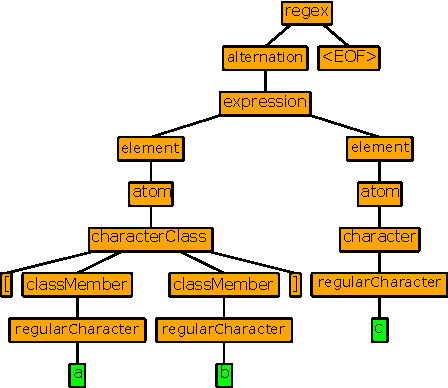
\includegraphics[width=0.7\textwidth]{tree.pdf}
    \caption{Parse tree for the pattern \texttt{\textbf{[ab]c}}.}
    \label{fig:parsetree}
\end{figure}

Thompson's algorithm works recursively by breaking down a regular expression into its fundamental sub-expressions, from which the NFA is built using the following set of rules:

\subsubsection{Literals}
A character literal is represented by an automaton of two states as in Figure \ref{fig:auto1}.

\begin{figure}[htpb]
\centering
\begin{tikzpicture}[->,>=stealth',shorten >=1pt,auto,node distance=3.5cm,scale = 1,transform shape]

  \node[state,initial] (s0) {$s0$};
  \node[state,accepting] (s1) [right of=s0] {$s1$};

  \path    (s0) edge                          node {$a$} (s1);

\end{tikzpicture}
\caption{Automaton for the pattern \texttt{\textbf{a}}.}
\label{fig:auto1}
\end{figure}
\subsubsection{Alternations}\label{epsremoval}
A new state \texttt{\textbf{p}} is added with epsilon transition to the start state of each alternation.

An epsilon transition from state \texttt{\textbf{p0}} to state \texttt{\textbf{p1}} is equivalent to adding all transitions of state \texttt{\textbf{p1}} and marking state \texttt{\textbf{p0}} as accept if \texttt{\textbf{state1}} was an accept state then, removing  state \texttt{\textbf{p1}} from the new automaton. Figure \ref{fig:auto2} shows the construction steps for the alternation between the two patterns \texttt{\textbf{a}} and \texttt{\textbf{x}}.

\begin{figure}[htbp]
\centering

\subcaptionbox{Automaton for the pattern \texttt{\textbf{a}}.}{
\begin{tikzpicture}[->,>=stealth',shorten >=1pt,auto,node distance=3.5cm,scale = 1,transform shape,baseline]

  \node[state,initial] (s0) {$s0$};
  \node[state,accepting] (s1) [right of=s0]{$s1$};

  \path    (s0) edge  node {$a$} (s1);

\end{tikzpicture}
}\hfill
\subcaptionbox{Automaton for the pattern \texttt{\textbf{x}}.}{
\begin{tikzpicture}[->,>=stealth',shorten >=1pt,auto,node distance=3.5cm,scale = 1,transform shape,baseline]

  \node[state,initial] (s0) {$s2$};
  \node[state,accepting] (s1) [right of=s0]{$s3$};

  \path    (s0) edge  node {$x$} (s1);

\end{tikzpicture}
}
\par\bigskip
\subcaptionbox{Automaton for pattern \texttt{\textbf{a|x}} with epsilon transitions.}{
\begin{tikzpicture}[->,>=stealth',shorten >=1pt,auto,node distance=2cm,scale = 1,transform shape, baseline]

  \node[state,initial] (p) {$p$};
  \node[state] (s0) [right of=p] {$s0$};
  \node[state,accepting] (s1) [right of=s0] {$s1$};
  \node[state] (s2) [below of=s0] {$s2$};
  \node[state,accepting] (s3) [right of=s2] {$s3$};

  \path    (p) edge                          node {$\epsilon$} (s0);
  \path    (p) edge                          node {$\epsilon$} (s2);
  \path    (s0) edge                          node {$a$} (s1);
  \path    (s2) edge                          node {$x$} (s3);
\end{tikzpicture}}\hfill
\subcaptionbox{Final Automaton for pattern \texttt{\textbf{a|x}} with epsilon transitions removed.}{
\begin{tikzpicture}[->,>=stealth',shorten >=1pt,auto,node distance=3.5cm,scale = 1,transform shape, baseline]

  \node[state,initial] (p) {$p$};
  \node[state,accepting] (s1) [right of=p] {$s1$};
  \node[state,accepting] (s3) [below of=s1] {$s3$};

  \path    (p) edge                          node {$a$} (s1);
  \path    (p) edge                          node {$x$} (s3);
\end{tikzpicture}}%

\caption{Automaton construction steps for alternation pattern \texttt{\textbf{a|x}}.}
\label{fig:auto2}
\end{figure}
\subsubsection{Concatenation}
The initial state of the first automaton becomes the initial state of the new NFA. The accepting states of the first automaton are marked as not accepting. Moreover, the accept states of the second automaton are the accept states of the new NFA. Finally, an epsilon transition is added from each accept state of the first automaton to the initial states of the second automaton. Figure \ref{fig:auto3} shows the concatenation between two patterns \texttt{\textbf{a}} and \texttt{\textbf{bc}}.

\begin{figure}[htpb]
\centering
\begin{tikzpicture}[->,>=stealth',shorten >=1pt,auto,node distance=3.5cm,scale = 1,transform shape]

  \node[state,initial] (s0) {$s0$};
  \node[state] (s1) [right of=s0]{$s1$};
  \node[state] (p1) [right of=s1] {$p1$};
  \node[state,accepting] (p2) [right of=p1] {$p2$};

  \path    (s0) edge                          node {$a$} (s1);
  \path    (s1) edge                          node {$b$} (p1);
  \path    (p1) edge                          node {$c$} (p2);

\end{tikzpicture}
\caption{Automaton to recognize the concatenation of the patterns \texttt{\textbf{a}} and \texttt{\textbf{bc}}.}
\label{fig:auto3}
\end{figure}
\subsubsection{Quantifiers}
\textbf{Kleene Star}: Row 1 in Table \ref{tab:regexquant} is the Kleene star \texttt{\textbf{*}} quantifier. It is an unbounded quantifier and is supported by adding a loop to the NFA. A new start state \texttt{\textbf{p}} is added with epsilon transition to the start state the automaton. Epsilon transitions from the accept states to \texttt{\textbf{p}} is added and \texttt{\textbf{p}} is marked as accept. An example for Kleene star is show in Figure \ref{fig:autoq1}.

\begin{figure}[H]
\centering
\begin{tikzpicture}[->,>=stealth',shorten >=1pt,auto,node distance=3.5cm,scale = 1,transform shape]

  \node[state,initial,accepting] (p) {$p$};
  \node[state,accepting] (s0) [right of=p]{$s0$};

  \path    (p) edge                          node {$a$} (s0);
  \path    (s0) edge [loop above] node {$a$} (s0);

\end{tikzpicture}
\caption{Automaton to recognize pattern \texttt{\textbf{a*}}.}
\label{fig:autoq1}
\end{figure}



\noindent
\textbf{Optional (Zero or one)}: Row 2 in Table \ref{tab:regexquant} is the Optional quantifier \texttt{\textbf{?}}. It is a bounded quantifier and is  equivalent to the alternation of an NFA and the empty string epsilon, e.g., \texttt{\textbf{a?}} is equivalent to \texttt{\textbf{a|\epsilon}}. Figure \ref{fig:autoq3} shows an example Automaton.


\begin{figure}[htpb]
\centering
\begin{tikzpicture}[->,>=stealth',shorten >=1pt,auto,node distance=3.5cm,scale = 1,transform shape]

  \node[state,initial,accepting] (p) {$p$};
  \node[state,accepting] (s0) [right of=p]{$s0$};

  \path    (p) edge node {$a$} (s0);

\end{tikzpicture}
\caption{Automaton to recognize pattern \texttt{\textbf{a?}}.}
\label{fig:autoq3}
\end{figure}

\noindent
\textbf{Plus (One or more)}: Row 3 in Table \ref{tab:regexquant} is the Plus quantifier \texttt{\textbf{+}}. It is an unbounded quantifier and is equivalent to concatenation of an NFA and Kleene star of the same NFA e.g \texttt{\textbf{a+}} is equivalent to \texttt{\textbf{aa*}}. Figure \ref{fig:autoq2} shows the example Automaton.

\begin{figure}[htpb]
\centering
\begin{tikzpicture}[->,>=stealth',shorten >=1pt,auto,node distance=3.5cm,scale = 1,transform shape]

  \node[state,initial] (s0) {$s0$};
  \node[state,accepting] (p)[right of=s0] {$p$};
  \node[state,accepting] (s1) [right of=p]{$s1$};

  \path    (s0) edge                          node {$a$} (p);
  \path    (p) edge                          node {$a$} (s1);
  \path    (s1) edge [loop above] node {$a$} (s1);

\end{tikzpicture}
\caption{Automaton to recognize pattern \texttt{\textbf{a+}}.}
\label{fig:autoq2}
\end{figure}

\newpage
\textbf{Counting}: Row 4 in Table \ref{tab:regexquant} is the counting quantifier. It's represented as alternation, e.g., \texttt{\textbf{a\{1,3\}}} is equivalent to \texttt{\textbf{a(a(a|\epsilon)|\epsilon)}} or \texttt{\textbf{a|aa|aaa}}. Figure \ref{fig:autoq4} shows the example automata.

\begin{figure}[H]
\centering
\begin{tikzpicture}[->,>=stealth',shorten >=1pt,auto,node distance=3.5cm,scale = 1,transform shape]

  \node[state,initial] (s0) {$s0$};
  \node[state,accepting] (s1) [right of=s0] {$s1$};
  \node[state,accepting] (s2) [right of=s1] {$s2$};
  \node[state,accepting] (s3) [right of=s2] {$s2$};

  \path    (s0) edge node {$a$} (s1);
  \path    (s1) edge node {$a$} (s2);
  \path    (s2) edge node {$a$} (s3);

\end{tikzpicture}
\caption{Automaton to recognize pattern \texttt{\textbf{a\{1,3\}}}.}
\label{fig:autoq4}
\end{figure}
\subsubsection{Character Classes}
\textit{Positive} character classes are treated the same way as alternations, e.g., NFA for character class \texttt{\textbf{[ax]}} is equivalent to NFA recognizing \texttt{\textbf{a|x}}. Figure \ref{fig:auto2} shows the resulting automaton.

\textit{Negative} Character Classes are equivalent to applying \texttt{\textbf{intersection}} between the \texttt{\textbf{anyChar}} wildcard automata and automata recognizing the \texttt{\textbf{Complement}} of the character class, e.g., \texttt{\textbf{[\textasciicircum ax]}} is equivalent to \texttt{\textbf{$\_ \cap [ax]$}}. Figure \ref{fig:auto4} shows the result automata where transitions are encoded in hex-decimal, and the language of the NFA is the ASCII character set. This operation is costly since the intersection uses the cross-product automaton construction method, which requires converting NFA to DFA first and is quadratic in the number of states.

\begin{figure}[htbp]

\begin{subfigure}[b]{0.5\textwidth}
\centering
\begin{tikzpicture}[->,>=stealth',shorten >=1pt,auto,node distance=3.5cm,scale = 1,transform shape]

  \node[state,initial] (s0) {$s0$};
  \node[state,accepting] (s1) [right of=s0]{$s1$};

  \path    (s0) edge  node {$[0x0-0x7F]$} (s1);

\end{tikzpicture}
\caption{Automaton for \texttt{\textbf{anyChar}}.}
\label{fig:auto41}
\end{subfigure}
\hfill
\begin{subfigure}[b]{0.5\textwidth}
\centering
\begin{tikzpicture}[->,>=stealth',shorten >=1pt,auto,node distance=5cm,scale = 1,transform shape]

  \node[state,initial,accepting] (s0) {$s0$};
  \node[state] (s1) [right of=s0]{$s1$};

  \path    (s0) edge  node {$[0x61-0x61]$} (s1);
  \path    (s0) edge  [bend right] node {$[0x78-0x78]$} (s1);

\end{tikzpicture}
\caption{Automaton for complement of \texttt{\textbf{[ax]}}.}
\label{fig:auto42}
\end{subfigure}\\


\begin{subfigure}[b]{\textwidth}
\centering
\begin{tikzpicture}[->,>=stealth',shorten >=1pt,auto,node distance=10cm,scale = 1,transform shape]

  \node[state,initial] (s0) {$s0$};
  \node[state,accepting] (s1) [right of=s0]{$s1$};

  \path    (s0) edge [bend left] node {$[0x0-0x60]$} (s1);
  \path    (s0) edge node {$[0x62-0x77]$} (s1);
  \path    (s0) edge [bend right] node {$[0x79-0x7F]$} (s1);
\end{tikzpicture}
\caption{Automaton for Intersection between Automaton \ref{fig:auto41} and Automaton \ref{fig:auto42}}.
\label{fig:auto43}
\end{subfigure}

\caption{Automaton Construction Steps for negative character class \texttt{\textbf{[\textasciicircum ax]}}. Char \texttt{\textbf{a}} is hex \texttt{\textbf{0x61}} and Char \texttt{\textbf{x}} is \texttt{\textbf{0x78}}.}
\label{fig:auto4}
\end{figure}


\subsection{NFA to DFA}\label{subsection:nfdtodfa}
After generating the NFA in the previous step, We use the Powerset construction algorithm to convert it into a DFA. The algorithm can transform any NFA into an equivalent deterministic automaton. However, there is one disadvantage: When the algorithm is applied to an NFA with $n$ states, the resulting DFA can have an exponentially larger number of states than $2^n$ \cite{dfasize}. We set an adjustable limit for the number of states the DFA can have to overcome this problem. We use a fallback library to handle this regular expression if the algorithm exceeds the limit.

\subsubsection{Powerset Construction}
The algorithm works by mapping associating each state in the DFA with a set of NFA states and it works as follows:
\begin{enumerate}
    \item The DFA's start state is the same as the NFA's start state, plus all states accessible via $\epsilon$-transitions.
    \item If a DFA state \texttt{\textbf{p}} corresponds to a set of NFA states \texttt{\textbf{S}}, then the transition from state p on a character \texttt{\textbf{c}} is as follows:
    \begin{enumerate}
        \item Let \texttt{\textbf{S1}} be the set of NFA states that can be reached by following a transition for character \texttt{\textbf{c}} from any of \texttt{\textbf{S}}'s states.
        \item The DFA state \texttt{\textbf{p}} transitions table row for character \texttt{\textbf{c}} is the DFA State \texttt{\textbf{q}} that corresponds to the set of states accessible via zero or more epsilon transitions from any state in \texttt{\textbf{S1}}.
    \end{enumerate}
\end{enumerate}
 

In our implementation, we modify the classic algorithm as follows:
 \begin{itemize}
     \item In NFA generation, we remove explicit $\epsilon$-transitions as we already get them in each NFA state transition table as outlined in sub-section \ref{epsremoval}. So we can skip the parts about $\epsilon$-transitions.
     \item Each transition we have is a range, not a single character, so the algorithm will not work when there are transitions with intersecting character ranges. To solve this, we iterate all the transition ranges in the NFA and transform them into a sorted set of non-intersecting ranges.
 \end{itemize}
 
Figure \ref{fig:ps1} shows an example conversion NFA to DFA for pattern \texttt{\textbf{xyz|xya}}.


\begin{figure}[htpb]
\begin{subfigure}[b]{\textwidth}
\centering
\begin{tikzpicture}[->,>=stealth',shorten >=1pt,auto,node distance=2cm,scale = 1,transform shape]

  \node[state,initial] (s0) {$s0$};
  \node[state] (s1) [right of=s0] {$s1$};
  \node[state] (s2) [right of=s1] {$s2$};
  \node[state,accepting] (s3) [right of=s2] {$s3$};
  \node[state] (s4) [below of=s1] {$s4$};
  \node[state] (s5) [right of=s4] {$s5$};
  \node[state,accepting] (s6) [right of=s5] {$s6$};

  \path    (s0) edge node {$x$} (s1);
  \path    (s0) edge node {$x$} (s4);
  
  \path    (s1) edge node {$y$} (s2);
  \path    (s2) edge node {$z$} (s3);
  
  \path    (s4) edge node {$y$} (s5);
  \path    (s5) edge node {$a$} (s6);
  

\end{tikzpicture}
\caption{NFA for pattern \texttt{\textbf{xyz|xya}}.}
\label{fig:ps11}
\end{subfigure}\hfill
\par\bigskip % force a bit of vertical whitespace

\begin{subfigure}[b]{\textwidth}
\centering
\begin{tikzpicture}[->,>=stealth',auto,node distance=2cm and 3cm,scale = 1,transform shape]

  \node[state,initial] (s0) {$\{s0\}$};
  \node[state] (s1) [right of=s0] {$\{s1,s4\}$};
  \node[state] (s2) [right of=s1] {$\{s2,s5\}$};
  \node[state,accepting] (s3) [right of=s2] {$\{s3\}$};
  \node[state,accepting] (s4) [below of=s3] {$\{s6\}$};

  \path    (s0) edge node {$x$} (s1);
  \path    (s1) edge node {$y$} (s2);
  \path    (s2) edge node {$z$} (s3);
  \path    (s2) edge node {$a$} (s4);
  
\end{tikzpicture}
\caption{DFA after applying powerset construction algorithm.}
\label{fig:ps12}
\end{subfigure}

\caption{Example conversion from NFA to DFA for pattern \texttt{\textbf{xyz|xya}}.}
\label{fig:ps1}
\end{figure}

\subsection{DFA Minimization}\label{dfamin}
The objective of DFA minimization is to convert a given DFA into an equivalent DFA with the fewest possible states. Two classes of states can be removed or merged from the original DFA without affecting the language it accepts. Without changing the language, it accepts the following types of states that can be removed or combined from the original DFA:

\begin{itemize}
    \item \textbf{Dead states}: states from which no accept state is reachable. We can remove these states.
    \item  \textbf{Unreachable states}: are the states that are not reachable from DFA's start state for any input. We can remove these states.
    \item \textbf{Non-distinguishable states}: are those that are not distinguishable from one another for any input. We can merge these states.
\end{itemize}

Dead and Unreachable states are easily removed in $O(n + m)$ where $n$ is the number of states, and $m$ is the number of transitions of the DFA. Several algorithms can identify and merge non-distinguishable states, e.g., Hopcroft's algorithm \cite{Hopcroftalgo} with worst-case time complexity of $O(ns log(n))$ where $n$ is the number of states and $s$ is the size of the alphabet.

In our implementation, we apply the removal of dead and unreachable states but not the merging of non-distinguishable states due to their time complexity. In our experiments, it did not have much impact on the type of patterns we focused on.

\section{Code Generation}
After generating the minimal DFA, the last step is to compiling it into efficient machine code. The \texttt{\textbf{CodeGen}} Module handles the conversion of the DFA to a more efficient representation and then Just-in-time (JIT) compiling the generated code, which speeds up regex matching at the cost of extra compilation time before matching.

Listing \ref{lst:dfainterpreted} shows simplified code for matching using interpreted DFA. The \texttt{\textbf{traverse}} function loops through the input string and, for each character, follows the transition table entry from the current state (Line 4). The matching fails if it does not find a matching entry (Lines 5-6). The matching succeeds if the current state is an accept state (Line 7). Otherwise, the loop continues with the next state (Line 8). 

The problem with the interpreted code is:
\begin{enumerate}
    \item It has lots of indirection and memory access for accessing the DFA state and transition table. Memory access wastes 100s of CPU cycles \cite{cpumemgap}.
    \item Data is not kept in CPU registers, and their contents are evicted regularly.
\end{enumerate}

\begin{listing}[htbp]
\inputminted[breaklines=true,frame=lines,linenos]{cpp}{code/interpretted.cpp}
\caption[Interpreted DFA Code]{Interpreted DFA Matching Code}
\label{lst:dfainterpreted}
\end{listing}

Due to the problems mentioned above with interpreted code, we use the \texttt{\textbf{CodeGen}} module to generate simple and efficient code for the DFA. The LLVM JIT compiler then compiles the generated code. The compiler returns a function pointer to the matching function we use later for matching the input text file.

The general algorithm for code generation and execution is as follows:
\begin{enumerate}
    \item The DFA is converted to a single function \texttt{\textbf{traverse}} that takes two parameters, the input string, and its length, and returns \texttt{\textbf{true}} if the pattern matches the input or \texttt{\textbf{false}} if no match is found or the input is finished before finding a match.
    \item The function consists of several code blocks:
    \begin{enumerate}
        \item Entry block for the string iterator initialization.
        \item A code block for each DFA state that consists of first a bound check if the input is finished, in which case it returns \texttt{\textbf{false}} otherwise, the next string character is loaded.
        \item After that, an \texttt{\textbf{if}} condition is generated for each transition out of the state. The condition transfers the control flow to the next DFA state or returns true if the transition goes to an accept state.
    \end{enumerate}
    \item If UTF-32 Encoding is enabled, three helper functions are added to the code. These functions are responsible for loading the correct code point from the input rather than a single character.
    \item LLVM JIT Compiler compiles the generated function code (LLVM IR). It then returns a function pointer to the traverse function.
\end{enumerate}

\subsubsection{C++ CodeGen}
Listing \ref{lst:cppex} shows the C++ code generated for pattern \texttt{\textbf{[a-z][0-9]}}. The generated code unrolls the DFA matching loop. Each state is represented as a labeled statement. Each transition is converted to a conditional statement where the condition is that the current character is in the transition range, and the body is a goto statement to the destination state label. Before listing the transitions for each state, a bounds check is added, and the next character in the input text is read. This representation eliminates any memory access for the DFA state and enables the compiler to eliminate a lot of indirection and dead code. In our implementation, we support C++ and LLVM IR code generation.

Before the last step in the code generation algorithm above, we use the C++ \texttt{\textbf{clang}} compiler to emit optimized LLVM IR before passing it to the JIT compiler.

\begin{listing}[htbp]
\inputminted[breaklines,frame=lines,linenos]{cpp}{code/ex.cpp}
\caption{Generated C++ Code for pattern \texttt{\textbf{[a-z][0-9]}}.}
\label{lst:cppex}
\end{listing}

Generating high-level C++ code is easy to implement and debug, but this approach has some disadvantages (1) The optimizing C++ compiler is slow compared to the LLVM Compiler. (2) Slow disk access is needed as the generated code must first be written to the disk as the C++ compiler \texttt{\textbf{clang}} does not support compiling an in-memory string buffer. Therefore, The JIT Compiler has to read the LLVM IR from the disk before being JITed which adds extra latency. For these reasons, most of the code-generation work focused on the LLVM backend for these reasons.

\subsubsection{LLVM CodeGen}
The \texttt{\textbf{CodeGen}} module generates code for the LLVM backend that is similar in structure to the code generated for C++ and follows the same general algorithm outlined above. However, it directly emits LLVM IR and is thus faster to JIT and optimize. The LLVM toolchain provides an excellent C++ API \cite{llvmapi} to help generate and validate the IR.

Let us walk through an example of going from a DFA to LLVM IR and using the LLVM toolchain to optimize and JIT the generated code. Figure \ref{fig:dfacodegenex} shows the DFA for pattern \texttt{\textbf{[a-z][0-9]}} that we will use as an example. The DFA consists of three states and two transitions.

\begin{figure}[H]
\centering
\begin{tikzpicture}[->,>=stealth',shorten >=1pt,auto,node distance=2.5cm,scale = 1,transform shape]

  \node[state,initial] (s0) {$s4$};
  \node[state] (s1) [right of=s1]{$s5$};
  \node[state,accepting] (s2) [right of=s1]{$s7$};

  \path    (s0) edge                          node {$[a-z]$} (s1);
  \path    (s1) edge                          node {$[0-9]$} (s2);

\end{tikzpicture}
\caption{DFA to recognize pattern \texttt{\textbf{[a-z][0-9]}}.}
\label{fig:dfacodegenex}
\end{figure}

Table \ref{tab:llvminst} lists the LLVM IR instructions and their meaning needed to understand the code generated.

{\renewcommand{\arraystretch}{1.5}% for the vertical padding
\begin{table}[H]
\centering
\small
\begin{tabularx}{\textwidth}{|l|X|}
\hline
Instruction        & Description  \\
\hline
\textbf{\%reg} & A (Static Single Assignment) SSA register named \texttt{\textbf{reg}}.\\
\hline
\textbf{alloca} & Allocate a variable on the stack.\\
\hline
\textbf{getelementptr} & Get the address of a sub element of an aggregate data structure (e.g., Arrays).\\
\hline
\textbf{load} & Load data from memory.\\
\hline
\textbf{store} & Write data to memory.\\
\hline
\textbf{br} & Branch to a different basic block in the current function which can be a conditional or unconditional branch. \\
\hline
\textbf{phi} & Implements the $\phi$ node in the SSA graph representing the function.\\
\hline
\textbf{and} & Performs a bitwise logical and.\\
\hline
\textbf{ret} & Returns control flow (and optionally a value) from a function back to the caller.\\
\hline
\textbf{icmp} &
Returns a boolean value or a vector of boolean values based on comparison of its integer operands.The first operand is the condition code indicating the kind of comparison to perform. Subset of possible condition codes are:\newline
\textbf{eq}: equal. \textbf{ne}: not equal. \textbf{ugt}: unsigned greater than.
\textbf{uge}: unsigned greater or equal. \textbf{ult}: unsigned less than. \textbf{ule}: unsigned less or equal.\\
\hline
\end{tabularx}
\caption[LLVM Instructions]{LLVM Instructions.}\label{tab:llvminst}
\end{table}}

Listing \ref{lst:llvmex} shows the complete code generated for the pattern. Line (1) defines the \texttt{\textbf{traverse}} function and its two parameters, an unsigned char pointer to input text, and the length of the input text.

Lines (2-5) describe the entry block in which the \texttt{\textbf{idx}} variable is defined and initialized to zero. This variable is used to traverse the input text. After that, an unconditional jump to the initial state starts the matching process.

Lines (6-8) define the initial state block, and we do bounds check if the current $idx >= n$. Line 9 is a conditional jump based on the comparison result before. If the comparison is \texttt{\textbf{true}}, it means the input is finished without a match, in which case we go to \texttt{\textbf{bounds\_then}} block and return \texttt{\textbf{false}}.

If the bounds check is \texttt{\textbf{false}}, we jump to block \texttt{\textbf{bonds\_cont}} Lines (12-20) where we first load the next character from the input text, increment the idx variable and then check the value of the character if it is in the range $[a - z]$. If the comparison succeeds, we jump to the next state block \texttt{\textbf{s5}}. Otherwise, we jump to the block \texttt{\textbf{s4\_nt}} and return \texttt{\textbf{false}} as no match is found.

Lines (23-41) repeat the same process but for the second state, and the check is for the range $[0-9]$. The only difference is that after matching that range, we jump to block \texttt{\textbf{s7}} that returns \texttt{\textbf{true}} indicating that a match is found. Figure \ref{fig:annocfg} shows an annotated Control Flow Graph (CFG) of the generated code.

In the next step, after generating the LLVM IR, The LLVM optimizer is used to validate and optimize the IR. The number and type of the applied optimization passes are configurable via the optimization level configuration option.

The LLVM code generator uses this optimization level to determine which optimization passes it should apply during the machine code generation. Each optimization level applies different optimizations that focus on either code size reduction or increased code performance. Table \ref{tab:optlevels} shows the default optimization levels shipped with LLVM. By default, we apply the \textbf{-O2} optimization level, which is a moderate level of optimization that enables most optimizations. The optimization level can be configured from the CLI as shown in Table \ref{tab:cliconf}.

{\renewcommand{\arraystretch}{1.1}% for the vertical padding
\begin{table}[H]
\centering
\small
\begin{tabularx}{\textwidth}{|l|X|}
\hline
Level        & Description  \\
\hline
\textbf{-O0} & Applies no optimizations. It compiles the fastest and generates the most debuggable code.\\
\hline
\textbf{-O2} & Is a moderate level of optimization that enables most optimizations.\\
\hline
\textbf{-O1} & Is a middle ground between -O0 and -O2.\\
\hline
\textbf{-Os} & Enables -O2 optimizations in addition to extra optimizations to reduce code size..\\
\hline
\textbf{-Oz} & Applies more optimizations to reduce code size than -Os.\\
\hline
\textbf{-O3} & Enables more optimizations than -O2 that may take longer to complete or may result in large code size (in an attempt to make the program run faster).\\
\hline
\end{tabularx}
\caption[LLVM Optimization Levels]{LLVM Optimization Levels.}\label{tab:optlevels}
\end{table}}


Applying the LLVM optimizer with Level \textbf{-O2} to the code generated yields the LLVM IR in Listing \ref{lst:llvmexs}. We notice the code size was halved from 42 to 21 lines. The number of code blocks was also halved, and common blocks were merged into the \texttt{\textbf{common.ret}} block. These results demonstrate the power of the LLVM optimizing compiler.

The last step after the optimization is passing the optimized IR to the JIT compiler that compiles it and returns a function pointer to the traverse function used for matching.

\begin{longlisting}
\inputminted[breaklines=true,frame=lines,linenos,fontsize=\small]{llvm}{code/irbefore.ll}
\caption{Generated LLVM Code for pattern \texttt{\textbf{[a-z][0-9]}} before LLVM optimizations.}
\label{lst:llvmex}
\end{longlisting}

\begin{listing}[H]
\inputminted[breaklines=true,frame=lines,linenos,fontsize=\small]{llvm}{code/irafter.ll}
\caption{Generated LLVM Code for pattern \texttt{\textbf{[a-z][0-9]}} after LLVM optimizations.}
\label{lst:llvmexs}
\end{listing}

\begin{figure}[H]
    \makebox[\textwidth][c]{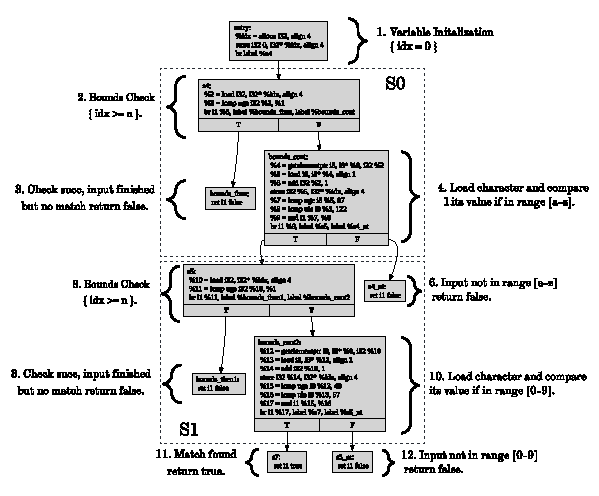
\includegraphics[width=1.42\textwidth]{code/cfga3.pdf}}%
    \caption{Annotated CFG for Generated LLVM Code for pattern \texttt{\textbf{[a-z][0-9]}} before LLVM optimizations.}
    \label{fig:annocfg}
\end{figure}

\section{Unicode}
Unicode is a standard that the Unicode Consortium created specifically to encode all of the characters in all of the world's writing systems. All modern database engines support Unicode characters, and users expect some kind of Unicode support. Therefore, Adding basic Unicode support to our prototype is a must-have feature. Also, since Unicode is an extensive character set, adding Unicode support helps test how well our prototype scales. Regular expression engines that are only adapted to handle small character sets, e.g., ASCII, will typically not scale well.

The Unicode Consortium has published guidelines \cite{unicodeguideline} on how regular expression engines can support Unicode. The guidelines specify three levels of Unicode support: Basic, Extended and Tailored.

Unicode level 1 support (Basic Unicode Support) defines the guidelines for minimal level for useful Unicode support. The results of regular expression matching at this level are not country or language-dependent. To accomplish complete Unicode processing at this level, the user of the regular expression engine would need to define more complicated regular expressions. A regular expression engine claiming conformance with Unicode level one must support:

\begin{enumerate}
    \item \textbf{Hex Notation}: An implementation must provide a means for expressing any Unicode code point (from U+0000 to U+10FFFF) using the hexadecimal code point encoding to meet these criteria.
    \item \textbf{Properties}: Unicode properties provide a convenient way to construct character classes of groups of code points specified by Unicode. E.g., Unicode general category property allows the user to express a category in a regular expression, such as "upper case letter" which encompasses all characters categorized as upper case letters in all of the world's writing systems.
    \item \textbf{Subtraction and Intersection}: An implementation must provide mechanisms for the union, intersection, and set-difference of sets of characters within regular expression character class expressions.
    \item \textbf{Simple Word Boundaries}: An engine supporting the test for word boundaries, e.g., the pattern \textbf{\textbackslash b} must be extended to include characters with the alphabetic property, characters from the Unicode decimal general category, zero-width joiners, or zero-width non-joiners.
    \item \textbf{Simple Loose Matches}: An engine supporting case-less matching must be extended to include at the very least the simple, default Unicode case-insensitive matching. Also, if it supports case conversions, it shall provide at least the simple, default Unicode case folding.
    \item \textbf{Line Boundaries}: A regular expression engine that supports line boundaries must support CRLF, LF, CR, NEL (U+0085), PARAGRAPH SEPARATOR (U+2029), and LINE SEPARATOR (U+2028).
    \item \textbf{Code Points}: An essential requirement is that Unicode text is semantically interpreted by code point rather than code unit.
\end{enumerate}

Unicode level 2 support for regular expression engines is referred to as Unicode extended support. The criteria for Unicode level 2 support are requirements to meet user expectations for Unicode character sequences. The primary needs for this level of support are support for canonical equivalence, extended grapheme clusters, and improved word boundary detection.

Unicode level 3 defines the specifications for tailored regular expression support. A regular expression engine can be tailored for a given area and utilized by specific groups of end-users.

Our prototype did not aim for a complete Unicode Level 1 support due to time constraints. We implemented only requirement seven \textbf{Code Points}, that is, that Unicode text is interpreted semantically by code points, not code units. Adding support for requirements (1-3) is an easy task and would primarily require parser grammar changes. There is little to no support for either Level 2 or Level 3. Most of this is due to the features being either complex/challenging to develop or, at the very least, extremely difficult to implement without losing performance.

In our prototype, we support two modes Unicode modes for matching: UTF-8 and UTF-32. We assume for both modes that both the pattern and input string are UTF-8 encoded (which includes ASCII).

\subsection{UTF-32}
We implemented this as the first step toward supporting Unicode in our prototype. 
In UTF-32 mode, the DFA generated matches full code points, and the logic for reading a full code point from the input text is handled outside the DFA loop by helper methods, effectively making the alphabet of the DFA the full Unicode range \texttt{\textbf{[0x000000-0x1FFFFF]}}. Figure \ref{fig:utf32exdfa} shows an example DFA to match the sterling character \texttt{\textbf{\textsterling}} (\textbackslash u00A3).

\begin{figure}[H]
\centering
\usetikzlibrary{fit}
\begin{tikzpicture}[->,>=stealth',shorten >=1pt,auto,node distance=2.5cm,scale = 1,transform shape]

  \node[state,initial] (s0) {$s0$};
  \node[state,accepting] (s1) [right of=s1]{$s1$};

  \path    (s0) edge                          node {$0x000000A3$} (s1);

\end{tikzpicture}
\caption[DFA to recognize pattern \texttt{\textsterling}]{UTF-32 DFA to recognize pattern \texttt{\textsterling}.}
\label{fig:utf32exdfa}
\end{figure}

To handle UTF-32 character encoding, a helper function \texttt{\textbf{nextCodepoint}} is added in the code generation step. Listing \ref{lst:utf32nextbyte} shows C++ code to recognize the pattern \texttt{\textbf{\textsterling}} with UTF-32. This function takes as an input a UTF-8 encoded input text and the index of first byte of the code point. It returns a full Unicode code point.

The function starts by loading the first byte in the text and then calls another helper function \texttt{\textbf{getLength}} that determines the number of bytes of the code point. As per Table \ref{tab:utf8}, the prefix of the first byte determine the number of bytes of the code point. It then calls a third helper function \texttt{\textbf{readMultiByte}} that reads the next \texttt{\textbf{byteLen}} bytes and encodes them to return the code point. Finally, the \texttt{\textbf{idx}} variable is incremented by \texttt{\textbf{byteLen}} to point to the start of the next code point.

While UTF-32 is easy to implement and makes the DFA generation step easier and results in an overall smaller automata, It is space inefficient since, in DFA generation, we have to store each transition as a 32-bit Integer, and the repeated function calls and logic for reading the full code point is costly and impacts the performance. In Chapter \ref{chapter:evaluation}, we evaluate the performance of UTF-32 against UTF-8.

\begin{listing}[H]
\inputminted[breaklines=true,frame=lines,linenos,fontsize=\small]{cpp}{code/utf32.cpp}
\caption{Generated C++ code for the pattern \texttt{\textbf{\textsterling}} with UTF-32 encoding.}
\label{lst:utf32nextbyte}
\end{listing}

\subsection{UTF-8}
UTF-8 is the default encoding mode of the engine. In order to support UTF-8, the engine embeds the UTF-8 decoding mechanism as states inside the DFA. The engine reads the regular expression as a sequence of bytes. It then generates a state for each byte resulting in a ByteDFA with an alphabet of $[0x0 - 0xFF]$.

As a demonstration of the DFA generation for UTF-8, Let us use the pattern ``\texttt{9\textvisiblespace \textsterling}" as an example. This pattern matches the digit nine followed by a space character then a sterling pound character. This pattern corresponds to the following sequence of code points \texttt{\textbf{\textbackslash u0039\textbackslash u0020\textbackslash u00A3}}. These code points are equivalent to the following UTF-8 byte sequences \texttt{\textbf{0x39 0x20 0xC2 0xA3}}. The engine reads the pattern as a sequence of bytes and generates a DFA with a single state representing each code unit (byte). Figure \ref{fig:utf8exdfa} shows the resulting DFA. The highlighted part shows the states that recognize the sterling pound code point.

At matching time, the matching function reads the input text one byte at a time, similar to a regular DFA without Unicode. This approach results in bigger DFAs but is faster and more space-efficient than UTF-32, as all the transitions are only a single byte, and there are no extra function calls.

\begin{figure}[htbp]
\centering
\begin{adjustbox}{width=1.1\textwidth,center=\textwidth}
\begin{tikzpicture}[->,>=stealth',shorten >=1pt,auto,node distance=2.5cm,scale = 1,transform shape]

  \node[state,initial] (s0) {$s0$};
  \node[state] (s1)[right of=s0] {$s1$};
  \node[state] (s2) [right of=s1]{$s2$};
  \node[state] (s3) [right of=s2]{$s3$};
  \node[state,accepting] (s4) [right of=s3]{$s4$};
  \node[draw,dotted,fit=(s2) (s3) (s4)] {};

  \path    (s0) edge                          node [scale=0.7] {$0x39$} (s1);
  \path    (s1) edge                          node [scale=0.7] {$0x20$} (s2);
  \path    (s2) edge                          node [scale=0.7] {$0xC2$} (s3);
  \path    (s3) edge                          node [scale=0.7] {$0xA3$} (s4);

\end{tikzpicture}
\end{adjustbox}
\caption{DFA to recognize pattern \texttt{9\textvisiblespace \textsterling} with UTF-8.}
\label{fig:utf8exdfa}
\end{figure}


\subsubsection{Character Ranges}
Embedding UTF-8 decoding inside the byte DFA raises issues with character classes that include ranges. To demonstrate the issue, let us say we want to match any Cyrillic character; we can do so with the pattern \texttt{\textbf{[\textbackslash u0400-\textbackslash u04FF]}}. The set of allowed bytes for this range can be expressed as a sequence of byte ranges: $\langle0xD0-0xD3\rangle \langle0x80-0xBF\rangle$. We can achieve this by simply encoding the boundaries \texttt{\textbf{\textbackslash u0400}} is encoded as $\langle0xD0 \; 0x80\rangle$ and \texttt{\textbf{\textbackslash u04FF}} is encoded as $\langle0xD3 \; 0xBF\rangle$ then we can create ranges from each corresponding pair of bytes: $0xD0 \rightarrow 0xD3$ and $0xD3 \rightarrow 0xBF$.

Now, let us try to extend the range to include Cyrillic Supplementary characters. The pattern becomes \texttt{\textbf{[\textbackslash u0400-\textbackslash u052F]}}. Applying the same algorithm above,  \texttt{\textbf{\textbackslash u0400}} is encoded as $\langle0xD0 \; 0x80\rangle$ and \texttt{\textbf{\textbackslash u052F}} is encoded as $\langle0xD4 \; 0xAF\rangle$ and we get the following sequence of byte ranges: $\langle0xD0-0xD4\rangle \langle0x80-0xAF\rangle$. However, this range is not correct because this range doesn't capture many characters, for example, \texttt{\textbf{\textbackslash u04FF}} as its last byte, $0xBF$ isn't in the range $\langle0x80-0xAF\rangle$. Instead we would need two sequences of byte ranges:

\begin{figure}[H]
\centering
$\langle0xD0-0xD3\rangle \langle0x80-0xBF\rangle$\\
$\langle0xD4\rangle \langle0x80-0xAF\rangle$
\end{figure}


To overcome this issue, we adapted an algorithm developed by \citet{utf8-ranges} for the rust regex crate. The algorithm converts Unicode scalar values to equivalent ranges of UTF-8 bytes. Figure \ref{fig:dfabmp} shows the resulting DFA for basic multilingual plane (BMP) \texttt{\textbf{[\textbackslash u{0000}-\textbackslash u{FFFF}]}} character class after applying the algorithm. The DFA in the Figure is obtained by the partitioning the range to the following sequences of byte ranges:

\begin{figure}[H]
\centering
$\langle0x0-0x7F\rangle$\\
$\langle0xC2-0xDF\rangle \langle0x80-0xBF\rangle$\\
$\langle0xE0\rangle \langle0xA0-0xBF\rangle \langle0x80-0xBF\rangle$\\
$\langle0xE1-0xEC\rangle \langle0x80-0xBF\rangle \langle0x80-0xBF\rangle$\\
$\langle0xED\rangle \langle0x80-0x9F\rangle \langle0x80-0xBF\rangle$\\
$\langle0xEE-0xEF\rangle \langle0x80-0xBF\rangle \langle0x80-0xBF\rangle$
\end{figure}


\section{Literals Optimizations}\label{section:simdopt}
Searching for a pattern that consists only of string literals, e.g., \texttt{\textbf{foobar}} is a common use-case for regular expressions matching in databases. A fast and smart regular expression engine can detect these patterns and optimize the search algorithm. The key to optimizing the search for literals on modern CPUs is how fast we can identify a candidate for a match. That is why we use Single Instruction Multiple Data (SIMD) instructions when detecting a literal. SIMD instructions can examine up to sixty-four bytes in a single loop iteration, making it very fast.

In our implementation, we detect these simple literal patterns, e.g., \texttt{\textbf{\%foobar\%}}, and apply one of the two algorithms explained below based on the size of the pattern.

\begin{figure}[H]
\centering
\begin{adjustbox}{width=0.8\textwidth,center=\textwidth}
\begin{tikzpicture}[->,>=stealth',shorten >=1pt,auto,node distance=3cm and 1.5cm,scale = 1,transform shape]

  \node[state,initial] (s0) {$s0$};
  \node[state] (s3) [right of=s0]{$s3$};
  \node[state] (s2) [above of=s3]{$s2$};
  \node[state] (s1) [above of=s2]{$s1$};
  \node[state] (s4) [below of=s3]{$s4$};
  \node[state] (s5) [below of=s4]{$s5$};
  \node[state,accepting] (s6) [below of=s5]{$s6$};

  \node[state] (s7) [right of=s1]{$s7$};
  \node[state] (s9) [right of=s3]{$s9$};

  \node[state] (s10) [right of=s4]{$s10$};
  \node[state,accepting] (s8) [right of=s9]{$s8$};

  \path    (s0) edge   [bend left]            node [scale=0.85,sloped] {$0xee-0xef$} (s1);
  \path    (s0) edge   [midway,align=left]         node [scale=0.8,sloped] {$0xe1-0xec$} (s2);
  \path    (s0) edge                          node [scale=0.85,sloped] {$0xed$} (s3);
  \path    (s0) edge  [bend right=20]         node [scale=0.85,sloped] {$0xe0$} (s4);
  \path    (s0) edge  [bend right=20]         node [scale=0.85,sloped] {$0xc2-0xdf$} (s5);
  \path    (s0) edge  [bend right]            node [scale=0.85,sloped] {$0x0-0x7f$} (s6);

  \path    (s1) edge                          node [scale=0.85] {$0x80-0xbf$} (s7);
  \path    (s2) edge                          node [scale=0.85,sloped] {$0x80-0xbf$} (s7);

  \path    (s7) edge [bend left]              node [scale=0.85,sloped] {$0x80-0xbf$} (s8);
  \path    (s3) edge                          node [scale=0.85] {$0x80-0x9f$} (s9);
  \path    (s9) edge                          node [scale=0.85] {$0x80-0xbf$} (s8);
  \path    (s4) edge                          node [scale=0.85] {$0xa0-0xbf$} (s10);
  \path    (s10) edge [bend right=10]                        node [scale=0.85,sloped,above] {$0x80-0xbf$} (s8);
  \path    (s5) edge [bend right=40]             node [scale=0.85,sloped] {$0x80-0xbf$} (s8);


\end{tikzpicture}
\end{adjustbox}
\caption{DFA to decode valid UTF-8 code point for BMP range \texttt{\textbf{[\textbackslash u0000-\textbackslash uFFFF]}}.}
\label{fig:dfabmp}
\end{figure}

\subsection{EPSM Algorithm}
Exact Packed String Matching (EPSM) \cite{epsm} is a string matching algorithm that makes use of bit-parallelism by packing several characters into a bit-word and partitioning string S into chunks $S_i$. A packed pattern bit-word is compared to these bit-word-sized chunks. Shift and bitwise-and operations are performed to compare the text chunks with the pattern. The algorithm is based on four different search procedures applied based on the pattern length $m$. 

In our implementation, we implement the first search procedure EPSMa and we use it only for short patterns $(m <= 16)$ as its performance degrades as the length of the pattern increases. Under these limitations, EPSM is very fast and runs in $O(n + occ)$ where $occ$ is the number of occurrences of the pattern $p$ in the text $t$. The asymptotic run-time for the general case is $O(n \times m)$.

The pseudo-code of the EPSMa algorithm is shown in Algorithm \ref{alg:espma}. The algorithm starts with a processing phase (lines 3-8) on the prefix of the pattern of length $m' = min(m, \alpha/2)$ where $\alpha$ is the number of characters of the alphabet that fit in a single word, e.g., for 128-bit registers and $\gamma$ the number of bits per character = 8, $\alpha = 16$. If $m = m'$ the algorithm pre-processes and searches the whole pattern. Otherwise, the algorithm acts as a filter that searches for the occurrences of the prefix of length $m'$ then naively checking the whole occurrence of the pattern if an occurrence of the prefix is found. In the processing phase, the algorithm constructs an array $B$ of $m'$ strings each of length $\alpha$. The $i$-th string in array $B$ consists of $\alpha$ copies of the character $p_i$.

\begin{figure}[H]
\centering
\begin{bytefield}{16}
\bitheader{0,4,8,12,15} \\
\begin{leftwordgroup}{A:}
\bitbox{4}{\textbf{0011}} & \bitbox{4}{0111} & \bitbox{4}{\textbf{1011}} & \bitbox{4}{0000}
\end{leftwordgroup} \\
\end{bytefield}

\begin{bytefield}{16}
\bitheader{0,4,8,12,15} \\
\begin{leftwordgroup}{B: }
\bitbox{4}{\textbf{0011}} & \bitbox{4}{1011} & \bitbox{4}{\textbf{1011}} & \bitbox{4}{1111}
\end{leftwordgroup} \\
\end{bytefield}

\begin{bytefield}[bitwidth=3em]{4}
\bitheader{0-3} \\
\begin{leftwordgroup}{R:}
\bitbox{1}{1} & \bitbox{1}{0} & \bitbox{1}{1} & \bitbox{1}{0}
\end{leftwordgroup} \\
\end{bytefield}
    \caption{Example for \texttt{\textbf{wscmp(a,b)}} where $\alpha = 4$, $\gamma=4$ and $w = 16$.}
    \label{fig:wscmpex}
\end{figure}

For the searching phase, we define the word-size compare instruction (\texttt{\textbf{wscmp}}) that compares its two w-bit sized inputs where $w$ is the number of bits in a computer word  handled as a block of $\alpha$ characters. Figure \ref{fig:wscmpex} shows an example application of wscmp(A,B). This instruction is equivalent to the following specialized SIMD instructions:

\begin{figure}[H]
\centering
\begin{cminted}{c}
h = mm_cmpeq_epi8(a, b)
r = mm_movemask_epi8(h)
\end{cminted}
\end{figure}

\begin{algorithm}[H]
\small
\begin{algorithmic}[1]
\State \alpha \gets the number of characters that fit in a single word. \Comment{For 128-bit registers and 8 bits per character $\alpha = 16$}
\Function{EPSMa}{$p,m,t,n$} \Comment{pattern, pattern length, text, text length}
    \State $m' \gets min(\alpha/2, m)$
    \For{$i \gets 0$ to $m' - 1$}                    
       \For{$i \gets 0$ to $\alpha - 1$}
            \State $B[i] \gets p[i]$
       \EndFor
    \EndFor
    \For{$i \gets 0$ to $(n/\alpha) - 1$}
        \State $r \gets 1^\alpha$
        \For{$j \gets 0$ to $m' - 1$}
            \State $s_j \gets wscmp(T_i, B_j)$
            \State $r \gets r \& (s_j << j)$
        \EndFor
        \If{$m = m'$}
            \State report occurrences at $i\alpha + \{r\}$ where r = $\{k | \, 0 \leq i < \alpha$ and $r_k = 1\}$
        \Else
            \State check positions $i\alpha + \{r\}$ where r = $\{k | \, 0 \leq i < \alpha$ and $r_k = 1\}$
        \EndIf
        \For{$j \gets 0$ to $m - 2$}
            \State check positions $(i + 1)\alpha - j$
        \EndFor

    \EndFor

\EndFunction
\end{algorithmic}
\caption{EPSMa Algorithm}\label{alg:espma}
\end{algorithm}

The searching phase (lines 9-23) processes the text $t$ in blocks of $\alpha$ characters. Therefore, Lets define  $N = \frac{n}{\alpha} - 1$ and the string $t$ of length $n$ as $T=T_0 T_1...T_N$. The instruction \texttt{\textbf{wscmp}} compares a block of the text $T_i$ is with the strings in the pre-processing array $B$. Let $s_j = wscmp(T_i, B_j) = b_0 b_1 ...b_{\alpha-1}$ for $0 \leq j < m'$ and $b_k = 1$ if and only if $T_{ik} = p_j$ for $0 \leq k < \alpha$. Lets also define $r = r_0 r_1...r_{m'-1}$ where $r_i = (s_i << i)$. It is apparent that the prefix of length $m'$ of the pattern $p$
occurs at the beginning at position $j$ of $T_i$ if and only if $r_j = 1$. If $m = m'$ then the whole pattern occurs and we can report the occurrences of the pattern at positions $i\alpha + \{r\}$ where r = $\{k | \, 0 \leq i < \alpha$ and $r_k = 1\}$. Otherwise, we know that at the same positions the prefix of the pattern matches and the algorithm checks the occurrences beginning at those positions. At the end, the algorithm naively checks the $m' - 1$ possible occurrences crossing the blocks $T_i$ and $T_i+1$.

The worst-case time complexity of the algorithm is $O(n \times m)$ as a naive check could be required for each position of the  However, for small patterns, the algorithm has a $O(n+occ)$ time complexity, where $occ$ is the number of occurrences of the pattern $p$ in the text $t$.


\subsection{Generic SIMD Algorithm}
This Generic SIMD algorithm \cite{simdalgo} is slower than the EPSMa algorithm but applies to patterns of any size. This algorithm's main idea is to use the equality of the pattern's initial and last characters as a predicate for a potential match. The pattern's two characters (first and last) are copied in two SIMD registers, $R1$ and $R2$, respectively. Then in each iteration of the algorithm, two chunks of strings are loaded into two other SIMD registers. The first chunk $C1$ is read from offset $i$ and the second chunk $C2$ is read from offset $i + k - 1$, where $k$ is the pattern length. Then the algorithm computes a vector expression $M1 = (R1 = C1)$ and $M2 = (R2 = C2)$ then $M = (M1 \& M2)$ that yields a bit mask where a set bit in the mask signals a position of potential match. At last, only at these positions exact comparisons of the pattern and the text are performed.

Figure \ref{fig:simdmatchalgo} shows an example application of the algorithm for pattern $p$ \textbf{foo} and text $t$ \textbf{hellofoo}. The algorithm returns a potential match at position $5$ in the pattern and a \texttt{memcmp} check is performed at this position.

\begin{figure}[H]
\centering
\begin{bytefield}[bitwidth=2em]{8}
\begin{leftwordgroup}{R1:}
\bitbox{1}{f} & \bitbox{1}{f} & \bitbox{1}{f} & \bitbox{1}{f}
& \bitbox{1}{f} & \bitbox{1}{f} & \bitbox{1}{f} & \bitbox{1}{f}
\end{leftwordgroup} \\
\end{bytefield}

\begin{bytefield}[bitwidth=2em]{8}
\begin{leftwordgroup}{C1:}
\bitbox{1}{h} & \bitbox{1}{e} & \bitbox{1}{l} & \bitbox{1}{l}
& \bitbox{1}{o} & \bitbox{1}{f} & \bitbox{1}{o} & \bitbox{1}{o}
\end{leftwordgroup} \\
\end{bytefield}

\begin{bytefield}[bitwidth=2em]{8}
\begin{leftwordgroup}{$M1 (R1 == C1)$:}
\bitbox{1}{0} & \bitbox{1}{0} & \bitbox{1}{0} & \bitbox{1}{0}
& \bitbox{1}{0} & \bitbox{1}{1} & \bitbox{1}{0} & \bitbox{1}{0}
\end{leftwordgroup} \\
\end{bytefield}


\begin{bytefield}[bitwidth=2em]{8}
\begin{leftwordgroup}{R2:}
\bitbox{1}{o} & \bitbox{1}{o} & \bitbox{1}{o} & \bitbox{1}{o}
& \bitbox{1}{o} & \bitbox{1}{o} & \bitbox{1}{o} & \bitbox{1}{o}
\end{leftwordgroup} \\
\end{bytefield}

\begin{bytefield}[bitwidth=2em]{8}
\begin{leftwordgroup}{C2:}
\bitbox{1}{l} & \bitbox{1}{l} & \bitbox{1}{o} & \bitbox{1}{f} & \bitbox{1}{o} & \bitbox{1}{o}
& \bitbox{1}{\_} & \bitbox{1}{\_}
\end{leftwordgroup} \\
\end{bytefield}

\begin{bytefield}[bitwidth=2em]{8}
\begin{leftwordgroup}{$M2 (R2 == C2)$:}
\bitbox{1}{0} & \bitbox{1}{0} & \bitbox{1}{1} & \bitbox{1}{0}
& \bitbox{1}{1} & \bitbox{1}{1} & \bitbox{1}{0} & \bitbox{1}{0}
\end{leftwordgroup} \\
\end{bytefield}

\begin{bytefield}[bitwidth=2em]{8}
\begin{leftwordgroup}{$M1 \, \& \, M2$:}
\bitbox{1}{0} & \bitbox{1}{0} & \bitbox{1}{0} & \bitbox{1}{0}
& \bitbox{1}{0} & \bitbox{1}{1} & \bitbox{1}{0} & \bitbox{1}{0}
\end{leftwordgroup} \\
\end{bytefield}

\caption{Example for SIMD string matching algorithm with 64-bit registers.}
\label{fig:simdmatchalgo}
\end{figure}

